\documentclass[twoside]{article}
\setlength{\oddsidemargin}{0 in}
\setlength{\evensidemargin}{0 in}
\setlength{\topmargin}{-0.6 in}
\setlength{\textwidth}{6.5 in}
\setlength{\textheight}{8.5 in}
\setlength{\headsep}{0.75 in}
\setlength{\parindent}{0 in}
\setlength{\parskip}{0.1 in}

\usepackage{url}
\usepackage{titlesec}
\setcounter{secnumdepth}{3}
\usepackage{palatino}
\usepackage{marginnote}
\usepackage{multirow}
\usepackage{easybmat,bigdelim,arydshln}
\usepackage[authoryear,round]{natbib}
\usepackage{amssymb,amsmath,amsthm,amsfonts}
\usepackage{mathtools}
%\usepackage{nicematrix}
\usepackage{arydshln}
\usepackage{caption}
\usepackage{hyperref}
\usepackage{tcolorbox}
\tcbuselibrary{skins, breakable, theorems}
\usepackage{newpxtext,newpxmath}
\usepackage{longtable}
\usepackage{enumitem}
\makeatletter

\let\bar\overline

\setlist[itemize]{topsep=0pt,leftmargin=10pt,itemsep=-0.2em}
\usepackage{xcolor}
\usepackage{tikz}
\usepackage{pgfplots}
\pgfplotsset{compat = newest}
\usetikzlibrary{patterns,decorations.pathreplacing,decorations.markings,fit,shapes.geometric,angles,quotes,arrows}
\usepgfplotslibrary{fillbetween}

\usepackage{ifthen}
\usepackage{tikz-3dplot}

\pgfdeclarelayer{ft}
\pgfdeclarelayer{bg}
\pgfsetlayers{bg,main,ft}

\hypersetup{
    colorlinks,
    citecolor=red,
    filecolor=black,
    linkcolor=violet,
    urlcolor=blue
}

\definecolor{myblue}{cmyk}{1,.72,0,.38}
\definecolor{mypurple}{cmyk}{.57,1,0,.58}
\definecolor{myred}{cmyk}{0,.88,.88,.58}
\definecolor{mygreen}{cmyk}{1,0,.69,.66}
\definecolor{myorange}{cmyk}{0,.58,100,.20}
\definecolor{glaucous}{rgb}{0.38, 0.51, 0.71}

\makeatletter
\renewcommand{\thefigure}{\thesection.\arabic{figure}}
\newtheoremstyle{indented}
  {3pt}% space before
  {3pt}% space after
  {\addtolength{\@totalleftmargin}{3.5em}
   \addtolength{\linewidth}{-3.5em}
   \parshape 1 3.5em \linewidth}% body font
  {}% indent
  {\bfseries}% header font
  {.}% punctuation
  {.5em}% after theorem header
  {}% header specification (empty for default)
\makeatother

\newcommand{\ind}{\perp\!\!\!\perp}

\theoremstyle{definition}
\newtheorem{defin}{Definition}[section] % Creates a new counter, number within section
\newtheorem{prt}[defin]{Remark} 
\newtheorem{prts}[defin]{Remarks} % Again share defin's counter
\newtheorem{exmp}[defin]{Example} % etc.
\newtheorem{exmps}[defin]{Examples}
\newtheorem*{note}{Note}
\tcbuselibrary{theorems}

% use counter*=defin to make each tcbtheorem share defin's counter

\newtcbtheorem[use counter*=defin, number within=section]{definition}{Definition}{enhanced, breakable,
    colback = white, colframe = red!55!black, colbacktitle = red!55!black, attach boxed title to top left = {yshift = -2.5mm, xshift = 3mm}, boxed title style = {sharp corners},fonttitle=\bfseries}{def}

\newtcbtheorem[use counter*=defin, number within=section]{theorem}{Theorem}{enhanced, breakable,
    colback = white, colframe = blue!45!black, colbacktitle = blue!45!black, attach boxed title to top left = {yshift = -2.5mm, xshift = 3mm}, boxed title style = {sharp corners},fonttitle=\bfseries}{thm}
    
\newtcbtheorem[use counter*=defin, number within=section]{proposition}{Proposition}{enhanced, breakable,
    colback = white, colframe = teal, colbacktitle = teal, attach boxed title to top left = {yshift = -2.5mm, xshift = 3mm}, boxed title style = {sharp corners},fonttitle=\bfseries}{prop}

\newtcbtheorem[use counter*=defin, number within=section]{lemma}{Lemma}{enhanced, breakable,
    colback = white, colframe = orange!80!black, colbacktitle = orange!80!black, attach boxed title to top left = {yshift = -2.5mm, xshift = 3mm}, boxed title style = {sharp corners},fonttitle=\bfseries}{lemma}

\newtcbtheorem[use counter*=defin, number within=section]{example}{Example}{enhanced, breakable,
    colback = white, colframe = yellow!60!black, colbacktitle = yellow!60!black, attach boxed title to top left = {yshift = -2.5mm, xshift = 3mm}, boxed title style = {sharp corners},fonttitle=\bfseries}{exmp}

\newtcbtheorem[use counter*=defin, number within=section]{assumption}{Assumption}{enhanced, breakable,
    colback = white, colframe = violet!60!white, colbacktitle = violet!60!white, attach boxed title to top left = {yshift = -2.5mm, xshift = 3mm}, boxed title style = {sharp corners},fonttitle=\bfseries}{assump}

\newtcbtheorem[use counter*=defin, number within=section]{algorithm}{Algorithm}{enhanced, breakable,
    colback = white, colframe = green!55!black, colbacktitle = green!55!black, attach boxed title to top left = {yshift = -2.5mm, xshift = 3mm}, boxed title style = {sharp corners},fonttitle=\bfseries}{algm}
%\newtcolorbox{example}[1]{enhanced, breakable, colback = white, colframe = orange!85!black, colbacktitle = orange!85!black, attach boxed title to top left = {yshift = -2.5mm, xshift = 3mm}, boxed title style = {sharp corners},fonttitle=\bfseries, title={Example: #1}}

\newtcbox{\myhl}[1][white]
  {on line, arc = 0pt, outer arc = 0pt,
    colback = #1!20!white, colframe = #1!50!black,
    boxsep = 0pt, left = 1pt, right = 1pt, top = 1pt, bottom = 1pt, boxrule = 0pt, bottomrule =0pt, toprule =0pt}
    
\newtcbox{\myhlrule}[1][white]
  {on line, arc = 0pt, outer arc = 0pt,
    colback = #1!20!white, colframe = #1!50!black,
    boxsep = 0pt, left = 1pt, right = 1pt, top = 1pt, bottom = 1pt, boxrule = 0pt, bottomrule =0.5pt, toprule =0.5pt}
%
% The following commands set up the lecnum (lecture number)
% counter and make various numbering schemes work relative
% to the lecture number.
%
\newcounter{lecnum}
\renewcommand{\thepage}{\thelecnum-\arabic{page}}
\renewcommand{\thesection}{\thelecnum.\arabic{section}}
\renewcommand{\theequation}{\thelecnum.\arabic{equation}}
\renewcommand{\thefigure}{\thelecnum.\arabic{figure}}
\renewcommand{\thetable}{\thelecnum.\arabic{table}}

\newcommand{\sidenotes}[1]{\marginnote{\raggedright\scriptsize#1}}
%
% The following macro is used to generate the header.
%
\newcommand{\lecture}[6]{
   \pagestyle{myheadings}
   \thispagestyle{plain}
   \newpage
   \setcounter{lecnum}{#1}
   \setcounter{page}{1}
   \noindent
   \begin{center}
   \framebox{
      \vbox{\vspace{2mm}
    \hbox to 6.28in { {\bf Econometrics
	\hfill \today} }
       \vspace{4mm}
       \hbox to 6.28in { {\Large \hfill Topic #1: #2  \hfill} }
       \vspace{2mm}
       \hbox to 6.28in { {\it #3 \hfill by #4} }
      \vspace{2mm}}
   }
   \end{center}
   \markboth{Week #1: #2}{Week #1: #2}

   {\bf Key points}: {#5}

   {\bf Disclaimer}: {\it #6}
   \vspace*{4mm}
}
%

\tikzset{-stealth-/.style={decoration={
  markings,
  mark=at position #1 with {\arrow{stealth}}},postaction={decorate}}}

  \tikzset{tangent/.style={
    decoration={
        markings,% switch on markings
        mark=
            at position #1
            with
            {
                \coordinate (tangent point-\pgfkeysvalueof{/pgf/decoration/mark info/sequence number}) at (0pt,0pt);
                \coordinate (tangent unit vector-\pgfkeysvalueof{/pgf/decoration/mark info/sequence number}) at (1,0pt);
                \coordinate (tangent orthogonal unit vector-\pgfkeysvalueof{/pgf/decoration/mark info/sequence number}) at (0pt,1);
            }
    },
    postaction=decorate
},
use tangent/.style={
    shift=(tangent point-#1),
    x=(tangent unit vector-#1),
    y=(tangent orthogonal unit vector-#1)
},
use tangent/.default=1}

\tikzstyle{terminator} = [rectangle, draw, thick, text centered, rounded corners, minimum height=2em]
\tikzstyle{process} = [rectangle, draw, thick, text centered, minimum height=2em]
\tikzstyle{decision} = [diamond, draw, thick, text centered, minimum width=3cm, minimum height=0.5cm]
\tikzstyle{data}=[trapezium, draw, thick, text centered, trapezium left angle=60, trapezium right angle=120, minimum height=2em]
\tikzstyle{arrow} = [thick,->,>=stealth]

\begin{document}
\lecture{20}{Random Forest}{}{Sai Zhang}{.}{The note is built on Prof. \hyperlink{http://faculty.marshall.usc.edu/jinchi-lv/}{Jinchi Lv}'s lectures of the course at USC, DSO 607, High-Dimensional Statistics and Big Data Problems.}
%\footnotetext{These notes are partially based on those of Nigel Mansell.}

\section{Motivation}
Denote by $m(\mathbf{X})$ the measurable nonparametric regression function with p-dimensional random vector $\mathbf{X}$ taking values in $[0,1]^p$. The Random Forest algorithm aims to learn the 
regression function in a non-parametric way based on the observations $\mathbf{x}_i \in [0,1]^p,y_i\in\mathbb{R},i=1,\cdots,n$, from the model 
$$
y_i = m(\mathbf{x}_i) + \epsilon_i
$$
where $\mathbf{X},\mathbf{x}_i,\epsilon_i,i=1,\cdots,n$ are independent, and $\left\{\mathbf{x}_i\right\}$ and $\left\{\epsilon_i\right\}$ are two sequences of identically distributed random variables. $\mathbf{x}_i$ is distributed identically as $\mathbf{X}$.

\paragraph*{Why Random Forest (RF)?} \textbf{RF} has gained significant popularity due to its
\begin{itemize}
    \item \myhl[myblue]{\textbf{High accuracy}}: \textbf{RF} consistently rank among the top performer, often surpassing more complex models
    \item \myhl[myblue]{\textbf{Robustness}}: \textbf{RF} are less subject to overfitting due to the ensemble nature leveraging multiple decision trees
    \item \myhl[myblue]{\textbf{Interpretability}}: \textbf{RF} provide rankings of feature importance
\end{itemize}

As illustrated in Figure \ref{fig:level2tree}, in a level-2 tree, each node (cell) defines the point where the current cell split and new cells are produced. The sets of features eligible for splitting cells at level $k-1$ are denoted as $\Theta_k\coloneq \left\{\Theta_{k,1},\cdots,\Theta_{k,2^{k-1}} \right\}$, where $\Theta_{k,s}\subset \left\{ 1,\cdots,p \right\}$.

\begin{figure}[ht]
    \begin{center}
        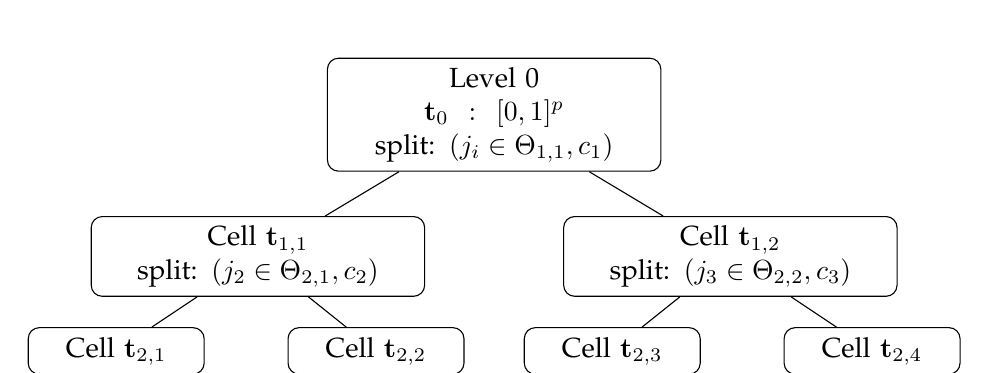
\begin{tikzpicture}[scale=1.2]
            % basics
            \node[draw,rectangle,rounded corners,text width=4cm,align=center] (a) at (0,2.5) {Level 0 \\ $\mathbf{t}_0:[0,1]^p$ \\ split: $\left(j_i \in \Theta_{1,1},c_1\right)$};
            \node[draw,rectangle,rounded corners,text width=4cm,align=center] (b1) at (-2.5,1) {Cell $\mathbf{t}_{1,1}$ \\ split: $\left(j_2 \in \Theta_{2,1},c_2\right)$};
            \node[draw,rectangle,rounded corners,text width=4cm,align=center] (b2) at (2.5,1) {Cell $\mathbf{t}_{1,2}$ \\ split: $\left(j_3 \in \Theta_{2,2},c_3\right)$};
            \node[draw,rectangle,rounded corners,text width=2cm,align=center] (c1) at (-4,0) {Cell $\mathbf{t}_{2,1}$};
            \node[draw,rectangle,rounded corners,text width=2cm,align=center] (c2) at (-1.25,0) {Cell $\mathbf{t}_{2,2}$};
            \node[draw,rectangle,rounded corners,text width=2cm,align=center] (c3) at (1.25,0) {Cell $\mathbf{t}_{2,3}$};
            \node[draw,rectangle,rounded corners,text width=2cm,align=center] (c4) at (4,0) {Cell $\mathbf{t}_{2,4}$};
            \draw[-] (a) -- (b1);
            \draw[-] (a) -- (b2);
            \draw[-] (b1) -- (c1);
            \draw[-] (b1) -- (c2);
            \draw[-] (b2) -- (c3);
            \draw[-] (b2) -- (c4);
        \end{tikzpicture}
    \end{center}
    \caption{Level-2 Tree Example}\label{fig:level2tree}
\end{figure}

Given any $T$ (and the associated splitting criterion) and $\Theta_{1:k}$, the tree estimate denoted as $\hat{m}_{T(\Theta_{1:k})}$ for a test point $\mathbf{c}\in [0,1]^p$ is defined as 
$$
\hat{m}_{T(\Theta_{1:k})}\left(\mathbf{c},\mathcal{X}_n\right) \coloneq \sum_{\left(\mathbf{t}_1,\cdots,\mathbf{t}_k\right)\in T(\Theta_{1:k})} \mathbf{1}_{\mathbf{c}\in\mathbf{t}_k}\left( \frac{\sum_{i\in \left\{i:\mathbf{x}_i\in \mathbf{t}_k\right\}} y_i}{\# \left\{i:\mathbf{x}_i\in\mathbf{t}_k\right\}} \right)
$$
where $\mathcal{X}_n\coloneq \left\{ \mathbf{x}_i,y_i \right\}^n_{i=1}$, the fraction is defined as $0$ when no sample is in the cell $\mathbf{t}_k$, and $\mathbf{1}_{\mathbf{c}\in\mathbf{t}_k}$ is an indicator function $=1$ if $\mathbf{c}\in\mathbf{t}_k$ and $=0$ otherwise.

\section{Chi et al. (2022): High Dimensional RFs}
Following \citet{chi2022asymptotic}, for a RF model where
\begin{itemize}
    \item a sequence of distinct $\Theta_{1:k}$ results in a distinct tree
    \item every set of available features $\Theta_{l,s}$, $l=1,\cdots,k$; $s=1,\cdots,2^{l-1}$
\end{itemize}

\paragraph*{Column subsampling} Define a \myhl[myblue]{\textbf{column subsampling}} procedure: $\Theta_{l,s},\forall l,s$ has $[\gamma_0p]$ distinct integers among $1,\cdots,p$, with $[\cdot]$ the ceiling function for some $0<\gamma_0\leq 1$. $\gamma_0$ is the predetermined constant parameter of column subsampling.
Introduce the boldface random mappings $\boldsymbol{\Theta}_{1:k}$, which are independent and uniformly distributed over all possible $\Theta_{1:k}$ for all integer $k$. Then random forests estimate for $\mathbf{c}$ with observations $\mathcal{X}_n$ is given by 
\begin{equation*}
    \mathbb{E}\left( \hat{m}_{T(\boldsymbol{\Theta}_{1:k})}\left(\mathbf{c},\mathcal{X}_n\right) \mid \mathcal{X}_n \right) = \sum_{\Theta_{1:k}} \mathbb{P} \left( \bigcap^k_{s=1} \left\{ \boldsymbol{\Theta}_s = \Theta_s \right\} \right) \hat{m}_{T(\Theta_{1:k})} \left(\mathbf{c},\mathcal{X}_n\right)
\end{equation*}
The expectation is taken over sets of available features.

\paragraph*{Observation resampling}
Let $A=\left\{a_1,\cdots, a_B\right\}$ be a set of subsamples with each $a_i$ consisting of $\lceil bn\rceil$ observations (indices) drawn without replacement from $\left\{1,\cdots,n\right\}$ for some positive integer $B$ and $0<b\leq 1$; in addition, each $a_i$ is independent of model training. The default values of $B$ and $b$ are $500$ and $0.632$\footnote{Or, $b=1$ but observations are drawn with replacement.}. Then the tree estimate using subsample $a$ is 
define as 
$$
\hat{m}_{T(\Theta_{1;k}),a}\left(\mathbf{c},\mathcal{X}_n\right) \coloneq \sum_{\left( \mathbf{t}_1,\cdots,\mathbf{t}_k \right)\in T(\Theta_{1:k})}\mathbf{1}_{\mathbf{c}\in\mathbf{t}_k}\left( \frac{\sum_{i\in a\cap \left\{i:\mathbf{x}_i\in\mathbf{t}_k\right\} }y_i}{\#\left(a\cap \left\{i:\mathbf{x}_i\in\mathbf{t}_k\right\}\right) } \right)
$$
the random forests estimate given $A$ is then 
$$
B^{-1}\sum_{a\in A}\mathbb{E}\left[\hat{m}_{T,a}\left(\boldsymbol{\Theta}_{1:k},\mathbf{c},\mathcal{X}_n \right) \mid \mathcal{X}_n\right] \coloneq B^{-1}\sum_{a\in A}\mathbb{E}\left[\hat{m}_{T(\boldsymbol{\Theta_{1:k}}),a}\left(\mathbf{c},\mathcal{X}_n\right)\mid \mathcal{X}_n\right]
$$

\paragraph*{CART-split criterion}
Given a cell $\mathbf{t}$, a subset of observation indices $a$ and a set of available features $\Theta \subset \left\{ 1,\cdots,p \right\}$, the CART-split is defined as 
\begin{equation}\label{eq:cart_split}
    \left(\hat{j},\hat{c}\right) = \arg\min_{j\in\Theta,c\in \left\{x_{ij}:\mathbf{x}_i\in\mathbf{t},i\in a\right\}} \left[ \sum_{i\in a \cap P_L}\left(\bar{y}_L-y_i\right)^2 + \sum_{i\in a\cap P_R}\left(\bar{y}_R-y_i\right)^2 \right]
\end{equation}
where 
\begin{align*}
    P_L & \coloneq \left\{ i: \mathbf{x}_i\in\mathbf{t},x_{ij}<c \right\} & P_R & \coloneq  \left\{ i: \mathbf{x}_i\in\mathbf{t},x_{ij}\geq c \right\}\\
    \bar{y}_L & \coloneq \sum_{i\in a \cap P_L}\frac{y_i}{\# \left(a\cap P_L\right)} & \bar{y}_R & \coloneq \sum_{i\in a \cap P_R}\frac{y_i}{\# \left(a\cap P_R\right)}
\end{align*}
The CART-split criterion conditional on the sample is a deterministic splitting criterion; conditioning on another sample leads to another deterministic splitting criterion. Define $\hat{T}_a$ as the sample tree growing rule that is associated with a splitting criterion following Eq. (\ref{eq:cart_split}), the tree estimates using $\hat{T}_a$ can be similarly defined as 
\begin{equation*}
    \hat{m}_{\hat{T}_a(\Theta_{1:k})} \left(\mathbf{c},\mathcal{X}_n\right) \coloneq \sum_{\left(\mathbf{t}_1,\cdots,\mathbf{t}_k\right)\in\hat{T}_a\left(\Theta_{1:k}\right)} \mathbf{1}_{\mathbf{c}\in\mathbf{t}_k}\left( \frac{\sum_{i\in \left\{i:\mathbf{x}_i\in \mathbf{t}_k\right\}}y_i}{\#\left\{i:\mathbf{x}_i\in\mathbf{t}_k\right\}} \right)
\end{equation*}
the definition is the same for $\hat{m}_{\hat{T}_a,a}$. Then the random forests estimate for a test point $\mathbf{c}\in [0,1]^p$ is given by 
\begin{equation*}
    B^{-1}\sum_{a\in A}\mathbb{E}\left( \hat{m}_{\hat{T}_a,a} \left(\boldsymbol{\Theta}_{1:k},\mathbf{c},\mathcal{X}_n\right) \mid \mathcal{X}_n\right)
\end{equation*}
where the average and conditional expectation correspond to the sample and column subsamplings respectively, and they are interchangeable.

\paragraph*{Bias-variance decomposition}
For a tree growing rule $T$ and $\Theta_{1:k}$, the population version is defined as 
\begin{equation}
    m^*_{T(\Theta_{1:k})}(\mathbf{c}) \coloneq \sum_{\left(\mathbf{t}_1,\cdots,\mathbf{t}_k\right)\in T(\Theta_{1:k})} \mathbf{1}_{\mathbf{c}\in\mathbf{t}_k}\mathbb{E}\left(m(\mathbf{X})\mid \mathbf{X}\in \mathbf{t}_k\right)
\end{equation}
for each test point $\mathbf{c}\in [0,1]^p$. And the $\mathbb{L}^2$ prediction loss for random forests is defined as 
\begin{equation}\label{eq:l2predictloss}
    \mathbb{E}\left[ m(\mathbf{X}) - B^{-1}\sum_{a\in A}\mathbb{E}\left( \hat{m}_{\hat{T}_a,a} \left(\boldsymbol{\Theta}_{1:k},\mathbf{X},\mathcal{X}_n\right)\mid \mathbf{X},\mathcal{X}_n \right) \right]^2
\end{equation}
if we use the full sample $a=\left\{1,\cdots,n\right\}$, and denote $\hat{T}_a$ and $\hat{m}_{\hat{T}_a,a}$ as $\hat{T}$ and $\hat{m}_{\hat{T}}$, the sample subsampling and average $B^{-1}\sum_{a\in A}\left(\cdot\right)$ in the random forests estimate are no 
longer needed, then Eq.(\ref{eq:l2predictloss}) can be simplified as 
\begin{equation*}
    \mathbb{E} \left[m(\mathbf{X})-\mathbb{E}\left(\hat{m}_{\hat{T}}\left(\boldsymbol{\Theta}_{1:k},\mathbf{X},\mathcal{X}_n\right) \mid \mathbf{X},\mathcal{X}_n\right)\right]^2
\end{equation*}
By Jensen's inequality and Cauchy-Schwarz inequality,
\begin{align*}
    &\frac{1}{2}\mathbb{E} \left[m(\mathbf{X}) - \mathbb{E}\left(\hat{m}_{\hat{T}} \left(\boldsymbol{\Theta}_{1:k},\mathbf{X},\mathcal{X}_n\right) \mid \mathbf{X},\mathcal{X}_n\right)\right]^2 \\
    \leq & \underbrace{\mathbb{E}\left[m(\mathbf{X}) - m^*_{\hat{T}} \left(\boldsymbol{\Theta}_{1:k},\mathbf{X}\right) \right]^2}_{\text{approximation error (squared bias)}} + \underbrace{\mathbb{E} \left[m^*_{\hat{T}}\left(\boldsymbol{\Theta}_{1:k},\mathbf{X}\right) -\hat{m}_{\hat{T}}\left(\boldsymbol{\Theta}_{1:k},\mathbf{X},\mathcal{X}_n\right)\right]^2}_{\text{estimation variance}}
\end{align*}

\section*{Consistency of RF Models}
For a cell $\mathbf{t}$ and its two daughter cells $\mathbf{t}'$ and $\mathbf{t}''$, define 
\begin{align*}
    \left(\mathbb{I}\right)_{\mathbf{t},\mathbf{t}'} \coloneq & \mathbb{P}\left(\mathbf{X}\in \mathbf{t}'\mid \mathbf{X} \in \mathbf{t}\right) \mathrm{Var} \left(m(\mathbf{X}) \mid \mathbf{X}\in\mathbf{t}'\right) + \mathbb{P}\left(\mathbf{X}\in \mathbf{t}''\mid \mathbf{X} \in \mathbf{t}\right)\mathrm{Var} \left(m(\mathbf{X}) \mid \mathbf{X}\in\mathbf{t}''\right) \\
    \left(\mathbb{II}\right)_{\mathbf{t},\mathbf{t}'} \coloneq & \mathbb{P}\left(\mathbf{X}\in \mathbf{t}'\mid \mathbf{X} \in \mathbf{t}\right) \left[\mathbb{E}(m(\mathbf{X})\mid \mathbf{X}\in\mathbf{t}') - \mathbb{E}(m(\mathbf{X})\mid \mathbf{X}\in \mathbf{t})\right]^2\\
    &+ \mathbb{P}\left(\mathbf{X}\in \mathbf{t}''\mid \mathbf{X} \in \mathbf{t}\right) \left[\mathbb{E}(m(\mathbf{X})\mid \mathbf{X}\in\mathbf{t}'') - \mathbb{E}(m(\mathbf{X})\mid \mathbf{X}\in \mathbf{t})\right]^2
\end{align*}
and $\left( \mathbb{I} \right)_{\mathbf{t,t}''}$ and $\left(\mathbb{II}\right)_{\mathbf{t,t}''}$ are defined similarly.

in this context, we assume the following regularity conditions:
\begin{itemize}
    \item \myhl[myblue]{\textbf{Absolutely continuous distribution}}: $f$, the density function of $\mathbf{X}$, is bounded away from $0$ and $\infty$
    \item \myhl[myblue]{\textbf{Covariates and model errors}}: assume $p=O(n^{K_0})$ for $K_0>0$, and there is a symmetric distribution around $0$ for $\epsilon_1$, s.t. $\mathbb{E}\left\vert \epsilon_1 \right\vert^q < \infty$ for sufficiently large $q>0$
    \item \myhl[myblue]{\textbf{Bounded regression functions}}: $\sup_{\mathbf{c}\in [0,1]^p}\left\vert m(\mathbf{c}) \right\vert \leq M_0$, for some $M_0>0$
    \item \myhl[myblue]{\textbf{Bounded regression functions}}
\end{itemize}

\newpage
\bibliographystyle{plainnat}
\bibliography{ref.bib}

\end{document}